%==============================================================================%
\chapter{Collecting Wi-Fi Data}\label{chapter:collection}
%==============================================================================%

From the literature review in Chapter \ref{chapter:literature}, we observed that  of all the technologies discussed, Wi-Fi seems to be the most promising one for our purposes.
We observed the advantages of Wi-Fi based data collection as,

\begin{itemize}[rightmargin=2em, leftmargin=2em]
  \itemsep-0.25em
  \item Universality as a standard technology globally,
  \item Independence from other types of data sources or infrastructure,
  \item High level of granularity both spatially and temporally,
  \item Possibility of passive data collection,
  \item Extreme ease of collection in terms of cost and effort and
  \item Scalability to cover study large areas.
\end{itemize}

Though it has its pitfalls in terms of intrusiveness resulting in risk to the privacy of the users, as well as bias and uncertainty, Wi-Fi provides us with a strong base framework for fulfilling the opportunity to design and collect a large, long-term and granular dataset which can be used for studying human activity.

In this chapter, we continue our research by looking at Wi-Fi technology closely to understand how it can be used to achieve the aforementioned goal.
We start by looking at the Wi-Fi specification \cite{ieee2016} and focus on the information available within the Wi-Fi probe requests.
We then design and implement a series of data collection exercises which collect probe requests in various location with increasing level of complexity for analysis.
We explore these datasets briefly to understand the usefulness of each set of information present in the probe requests along with the uncertainties in them.
We also introduce the `Smart Street Sensor' project - a national scale effort for collecting Wi-Fi data at high streets across the United Kingdom.
Finally we summarise the data collection procedure with a detailed look at the uncertainties in these datasets and draw conclusions for further lines of research into alleviating the uncertainty and noise so that the datasets can be used to estimate human activity with confidence.

%------------------------------------------------------------------------------%
\section{Wi-Fi as a Source of Data} \label{wifi-as-source-of-data}
%------------------------------------------------------------------------------%

Since the formation of `Wi-Fi alliance' in 1999 to hold the trademark, Wi-Fi (Wireless Fidelity) has become synonymous with the IEEE 802.11 standard based internet connectivity.
Today almost almost all devices use this standard to create and connect to local area networks wirelessly.
Due to its high fidelity and immense throughput up to 1 Gigabits per second, Wi-Fi has become the choice of technology for wirelessly transferring large amount data through networks.
The adoption of `smart' mobile devices Smartphones across the world has further cemented Wi-Fi's position as one of the most ubiquitous technologies which many people use every day.
In developed economies such as the UK, this has never been more true and having an infrastructure to serve and receive Wi-Fi signals greatly affects the ability to connect to the internet in many areas.
With close to 87\%\cite{deloitte2018} of the population carrying one or more of these smart devices with Wi-Fi capability, provision of Wi-Fi as a service has become essential for any place, thus making Wi-Fi (alongside mobile networks) one of the most used technologies to access the internet.

Though the end goal of internet connectivity is the same, Wi-Fi greatly differs from internet connectivity through mobile networks such 3G/4G.
The first difference is the range of the network: unlike mobile infrastructure where a single tower can serve mobile phones for miles, Wi-Fi is designed to be an extension of the wired networking, thus creating short range network with a range of 20 meters.
Due to this low-range and high throughput property, Wi-Fi is used primarily as a distributed infrastructure operated by owners of premises as a means to provide high speed connectivity to the users of these buildings as opposed to the large, national level, monolithic infrastructure that runs the mobile network.
This creates a situation where urban areas are populated by hundreds and thousands of these small area networks to which any mobile device can connect to.
Unlike the mobile service providers and their customers, these Wi-Fi networks and mobile devices don't trust each other with specialised hardware.
This creates a need for an introduction procedure - a sort of handshake between them - whereby they exchange information about themselves. 
Moreover since these mobile devices constantly move across these Wi-Fi networks, it becomes necessary for them to carry out these `handshake' processes regularly and frequently so that they can traverse between the networks without loss of connectivity.
This need for constant lookouts for new networks is solved by the `Probe requests'.

%------------------------------------------------------------------------------%
\subsection{Probe requests}
%------------------------------------------------------------------------------%

There have been numerous iterations and versions of the IEEE 802.11 standards but essentially all of them operate by exchanging packets of information called `datagrams' or `frames'.
These frames have the information that is being exchanged along with the meta data and information on the device that is sending them.
Some of these frames have special purposes: one such purpose is the `network discovery'.
The frames used for this purpose by the mobile device and the Access Point (AP) are called the 'probe request' and `probe response' respectively.
Though the actual information exchanged between these devices are usually encrypted, these probe requests are unencrypted and are accessible to any device which is listening.
The structure of a probe request is shown in Figure \ref{figure:collection:proberequest}.

\begin{figure*}
  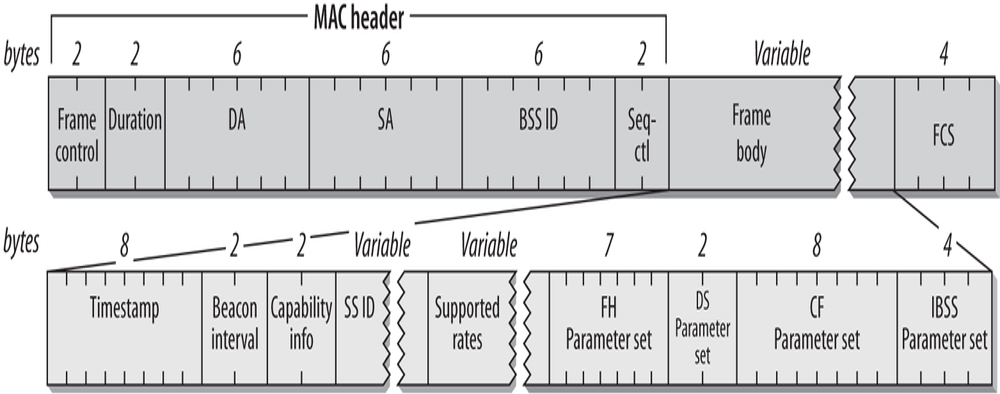
\includegraphics[width=0.9\textwidth,trim={0 -30 0 -10},clip]{images/probe-request-structure.png}
  \caption{Structure of a probe request frame. }
  \label{figure:collection:proberequest}
\end{figure*}
\marginnote[0.75cm]{\textit{Source: IEEE 802.11 specification}. DA - Destination Address. SA - Sender Address. BSSID - Broadcast or multicast address. FH - Frequency hopping. OS - Optional. CF - Contention free. DS - Direct Sequnce. }

We can observe that the fixed part of the mandatory frames are in the front; these show the identity of the mobile device generating the frame along with the identity of the AP that is receiving the frame.
There are additional meta data such as the sequence number of the frame, and controls denoting where the frame starts and ends.
There are also a number of variable information which can be used to transfer data.
For probe requests, the destination device is set as `broadcast' and the variable part usually contains the payload.
For probe request frames, this payload consists of `information elements' which has data regarding the capabilities of the device organised in units known as 'tags' or 'parameter sets'.
The significant information present in a probe request is detailed in Table \ref{table:collection:proberequest} and a full list of information available from a probe request is shown in the form of a sample probe request in appendix \ref{appendix:sampleprobe}

Essentially the above information is sent over and over by the mobile device which expects a reply from nearby APs so that it can keep a list of networks it can connect to.
This process is usually carried out even when the Wi-Fi is switched off in the operating system so that the connection times are faster once it is switched on.
Moreover operating systems use the replies they get for these probe requests and triangulate the device location with respect to the APs with location information on AP's collected through surveys or crowdsourcing, thus acting as a quick and easy localisation solution which along with the above makes this probing process almost non-stop. 

\begin{table}
  \footnotesize
  \begin{center}
    \begin{tabular}{lp{6.5cm}}
      \toprule
        Field & Notes\\
      \midrule
        \addlinespace[0.2cm]
        Source Address & Media Access Control (MAC) address\\
        Time stamp & Precise time at which the frame is received\\
        Received Signal Strength (dBm) & The strength of the received signal\\
        Length of the frame & Total length of the frame in bytes\\
        Duration of transmission & Time it took to transmit the frame in milliseconds\\
        Information Elements & List of various information about the device\\
        Known Networks & Name of networks that are already known to the device\\
      \bottomrule
    \end{tabular}
  \end{center}
  \caption{Significant information included in a probe request}
  \label{table:collection:proberequest}
\end{table}


%------------------------------------------------------------------------
\subsection{MAC address}
%------------------------------------------------------------------------------%
Media Access Control (MAC) address is a 6 byte unique identifier assigned to a device on a network.
It is similar to the Internet Protocol (IP) address but assigned at the interface controller level by the manufacturer of the device.
Although the IP address of a mobile device might change regularly, the MAC address usually remains the same for the lifetime of the device making it akin to a unique identifier of a device and therefore highly significant.
The MAC address has two parts: the first 2 bytes are known as the Organisationally Unique Identifier (OUI) and gives us information about the manufacturer of the network card.
Organisations need to register with IEEE to be assigned an OUI which they can use to generate a full MAC address;
the second 2 bytes are unique to device itself.
Together both form the full MAC address which is unique to every device globally.
The biggest draw for using Wi-Fi for mobility analysis comes from the fact that this globally unique identification is sent out regularly by mobile devices and can be collected passively through probe requests.

As we saw in our literature review, this also creates an immense risk in terms of infringement of privacy both for the manufacturer and the user.
Manufacturers of critical hardware components who do not want their unique MAC address to be publicised usually opt for registering a `private' OUI which will be neither given out to other manufacturers nor published publicly.
Users (their mobile devices) who don't want to be tracked using their MAC addresses use a temporary MAC address which is unique only to the local network - a `local' OUI rather than using a `global' OUI for unencrypted communications and switch to their original MAC address when a trusted encrypted connect has been established.
This lack of uniqueness can be inferred from the second character of the MAC address being E, A, 2 or 6.
Though this provides reasonably better privacy to the mobile users it also limits our ability to use the MAC address from the probe requests as in previous studies conducted with Wi-Fi.
It is important to note that this is not a security measure, but rather an exception made available by IEEE 802.11 for assigning temporary addresses in ad-hoc networks which has been used by most modern operating systems.

Essentially, there are two types of MAC addresses based on whether they have a public OUI or a private OUI.
This distinction does not affect their uniqueness or usefulness in mobility research but hinders us from knowing about the device from the MAC address.
There are also two types of MAC addresses based on them being unique globally or just in the local network.
This distinction affects the feasibility of using the MAC addresses for device tracking or for studying movement of the users.

To summarise the above, we looked at the IEEE 802.11 standard to examine the significance and nature of the `probe requests' which are constantly broadcast by mobile devices.
We identified information present in these probe requests which is relevant to our study and examined the uniquely identifiable MAC address field in detail.
We found that though a MAC address provides a way to globally identify a mobile device from the probe requests it generates, this field can often be masked by using locally assigned addresses.
We also observe that there is other relevant information which, when combined, can provide us with an alternative to solely using MAC addresses.

%==============================================================================%
%==============================================================================%
\section{Initial Experiments}
%==============================================================================%

With our theoretical understanding of the Wi-Fi standard and its capabilities, we move on to looking at the Wi-Fi landscape in real-world.
We achieve this by designing small independent experiments where we record the Wi-Fi probe requests within controlled conditions along with the knowledge of the ambient population of the field of measurement. 
We then look at the collected probe requests, examine them in detail to look at their properties, aggregate them to footfall counts and compare them with the real-world counts to get a overall idea of how well they translate into real counts.
The aim of these experiments to know more about the probe requests data and pick out the uncertainties and opportunities present in them.
The objectives here are,

\begin{enumerate}
  \setlength{\itemindent}{2em}
  \itemsep-0.25em
   \item Design a simple method to collect probe requests.
  \item Select locations with different levels of complexity.
  \item Collect real-world data through manual counting.
  \item Analyse the probe requests to extract useful information.
\end{enumerate}

%------------------------------------------------------------------------------%
\subsection{Experiment Design}
%------------------------------------------------------------------------------%

The first step was to design a simple method to collect Wi-Fi probe requests.
We accomplish by utilising the application - \textit{tshark} \cite{wireshark2} on a regular laptop.
First we put the Wi-Fi module of the laptop in `Monitor mode' where it behaves as a wireless access point.
Then we run tshark to collect the data in CSV format using the following command under a shell.

\begin{minted}{bash}
#! /bin/bash
tshark \
  -I -i en0 \
  -T fields \
  -E separator=, \
  -E quote=d \
    -e frame.time \
    -e frame.len \
    -e wlan_radio.signal_dbm \
    -e wlan_radio.duration \
    -e wlan.sa_resolved \
    -e wlan.seq \
    -e wlan.tag.length \
    -e wlan.ssid \
  type mgt subtype probe-req and broadcast
\end{minted}

The fields marked with \textit{-e} correspond to time stamp when the packet was received, total length of the packet, reported signal strength, duration for which the packet was transmitted, the MAC address of the source device, sequence number of the packet assigned by the source device, length of the tags attached to the packet and the network for which the probe request is being sent for.
The manufacturer information is extracted from the \textit{wlan.sa\_resolved} field into a separate column and the original field is hashed using the SHA256 algorithm implemented in R.
In addition to this, the pedestrians next to the sensor were counted manually by the surveyor.

%------------------------------------------------------------------------------%
\subsection{Living room}
%------------------------------------------------------------------------------%

\begin{marginfigure}
  \forcerectofloat
  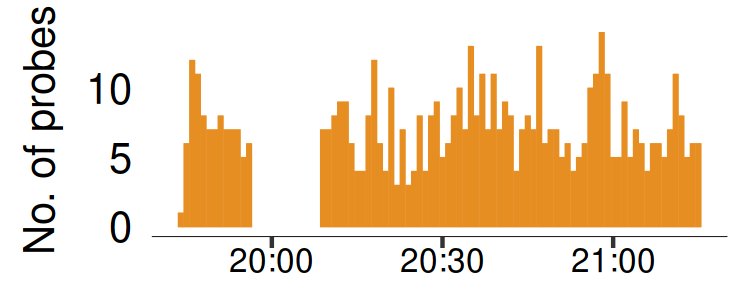
\includegraphics{images/home-total-count.png}
  \caption{Number of probe requests collected every minute on 15 October 2017}
  \label{figure:collection:home:total}
\end{marginfigure}

The first set of experiment was conducted with the laptop in the researcher's living room.
The primary aim of this experiment to collect an initial set of probe requests to understand the information in them.
The living room had 2 Wi-Fi enabled device - a motorola phone and an android tv 
The house had 2 more phones - iPhone and a Samsung phone.
Probe requests were collected on 15 Nov 2015 from 19:44 to 21:15 with a gap of 15 minutes in between.
We collected around 3000 probe requests at the rate of 38 requests per minute.

The first step was to look to convert these probe requests to number of devices by aggregating by the MAC addresses.
This results are shown in Figure \ref{figure:collection:home:total} which shows the number of unique MAC addresses detected every minute.
We see that aggregating by MAC addresses shows around 7 devices on average every minute around the sensor.
Though this might be true when considering noise from outside the room, it also reports around 211 unique MAC addresses overall these cannot be possibly generated by unique devices.
These unique addresses must have been caused by the randomisation process thus confirming that MAC addresses alone is not enough to convert the probe requests in to unique devices.

After this we looked at the resolved OUIs from the data.
There are 24 different vendors.
This is more than what we expected showing that these ones must be clearly coming from outside the room / house.
We need to find a way to look at the
We need to look at signal strength which can show how far the device is.
we look at the compression ration of MAC vs probes which shows the amount of randomisation.
Since we hashed the mac address there is no way of finding out. we need to keep the OUI part which is independent from vendor. Not all local OUIs are private.
Compex, Google and local addresses are randomising.
Samsung is tricky since we know that samsung phones don't randomise. we need to look into this more to see if it is randomisation.
nvidia, amazon, azurewav does not randomise.

%:read !tail -n +7 ./analysis/data-collection/vendor-tables.txt | head -n -3
\begin{table}
\footnotesize
\begin{center}
  \begin{tabular}{lrrrrrrrr}
  \toprule
  Vendor & Probe & MAC & Signal & Frame & Dura-& Tags & SSID & Sequence \\ 
  & request & address & strength & length &  tion &  &  & numbers \\ 
  \midrule
  AmazonTe &  101 &   1 & -80.53 &   4 &   4 &   5 &   3 & 101 \\ 
  Apple    &   77 &   7 & -86.29 &   4 &   4 &   9 &   4 &  77 \\ 
  ArrisGro &    7 &   1 & -91.71 &   1 &   1 &   1 &   1 &   7 \\ 
  Azurewav &  215 &   4 & -87.82 &   3 &   3 &  12 &  10 & 213 \\ 
  CompexPt &   75 &  28 & -88.17 &   3 &   3 &   5 &  29 &  74 \\ 
  CompexUs &    4 &   1 & -87.25 &   3 &   3 &   3 &   4 &   4 \\ 
  Dedicate &    2 &   1 & -92.50 &   1 &   1 &   1 &   1 &   2 \\ 
  Fn-LinkT &   64 &   1 & \textcolor{red}{-60.58} &   2 &   2 &   6 &   1 &  64 \\ 
  Google   & 1347 &  76 & \textcolor{red}{-69.14} &   4 &   5 &  41 &   6 & 1157 \\ 
  HuaweiTe &   11 &   3 & -87.91 &   3 &   3 &   3 &   1 &  11 \\ 
  IntelCor &   25 &   2 & -84.04 &   3 &   3 &   4 &   3 &  25 \\ 
  LenovoMo &    1 &   1 & -93.00 &   1 &   1 &   1 &   1 &   1 \\ 
  LgElectr &    1 &   1 & -90.00 &   1 &   1 &   1 &   1 &   1 \\ 
  Microsof &    3 &   1 & -90.00 &   1 &   1 &   1 &   2 &   3 \\ 
  Nvidia   &   65 &   1 & -82.91 &   2 &   2 &   4 &   2 &  65 \\ 
  OneplusT &    3 &   1 & -86.67 &   2 &   2 &   2 &   2 &   3 \\ 
  Pepwave  &    4 &   4 & -90.00 &   1 &   1 &   1 &   1 &   4 \\ 
  Sagemcom &    3 &   1 & -88.67 &   1 &   1 &   1 &   1 &   3 \\ 
  SamsungE &  655 &  27 & -83.81 &  26 &  26 &  54 &  23 & 621 \\ 
  SonyMobi &   56 &   2 & -78.66 &   2 &   2 &   2 &   1 &  56 \\ 
  TctMobil &    1 &   1 & -90.00 &   1 &   1 &   1 &   1 &   1 \\ 
  Tp-LinkT &   31 &   1 & -86.16 &   1 &   1 &   3 &   1 &  31 \\ 
  Wisol    &  143 &   3 & -71.91 &   4 &   5 &   6 &   3 & 142 \\ 
  XiaomiCo &    3 &   2 & -88.67 &   2 &   2 &   3 &   2 &   3 \\ 
  Unknown  &  110 &  40 & -88.86 &  19 &  18 &  21 &   5 &  90 \\ 
  \bottomrule
  \end{tabular}
\end{center}
\caption{Number of unique values present in each field captured from the probe requests for each Vendor OUI}
\label{table:collection:proberequest}
\end{table}

We then look at the average signal strength.
Only two of the vendors have averages less than 70 showing the only two devices that are in the room.
Rest of the devices are more than 80. Showing the exponential decay of the signal strength as we cross walls.
Signal strength can be a good indicator to isolate devices based on their distance from the sensor.
Figure shows the distribution of the signal strengths, we can clearly see inside and outside the room from the distribution.
We found that it is not enough.

We then look at all the other information we collected from the probe requests and see how they compare to the MAC address for aggregating.
We see length, duration provides provides better aggregation fields than MAC whent he addresses are randomised.
The logic behind this is that since the phones are essentially sending the same information over and over with just changed MAC addresses (which is of fixed length) same phones should be sending packets of same length.
We also see that duration of the transfer being a function of the length of the packet almost same as unique as the length.
We can say there is no additional information encoded within the duration more than the length of the packet.
Tags and SSIDs though looked promising, doesn't give us enough unique finger print for the device.
Tags don't have much uniqueness device-wise and SSID information is sparse.
This is because of most of the devices don't have this field 66\% of local OUIs , 50\% of Google and 38\% of samsung probes dont have any SSID information.

\begin{figure}
  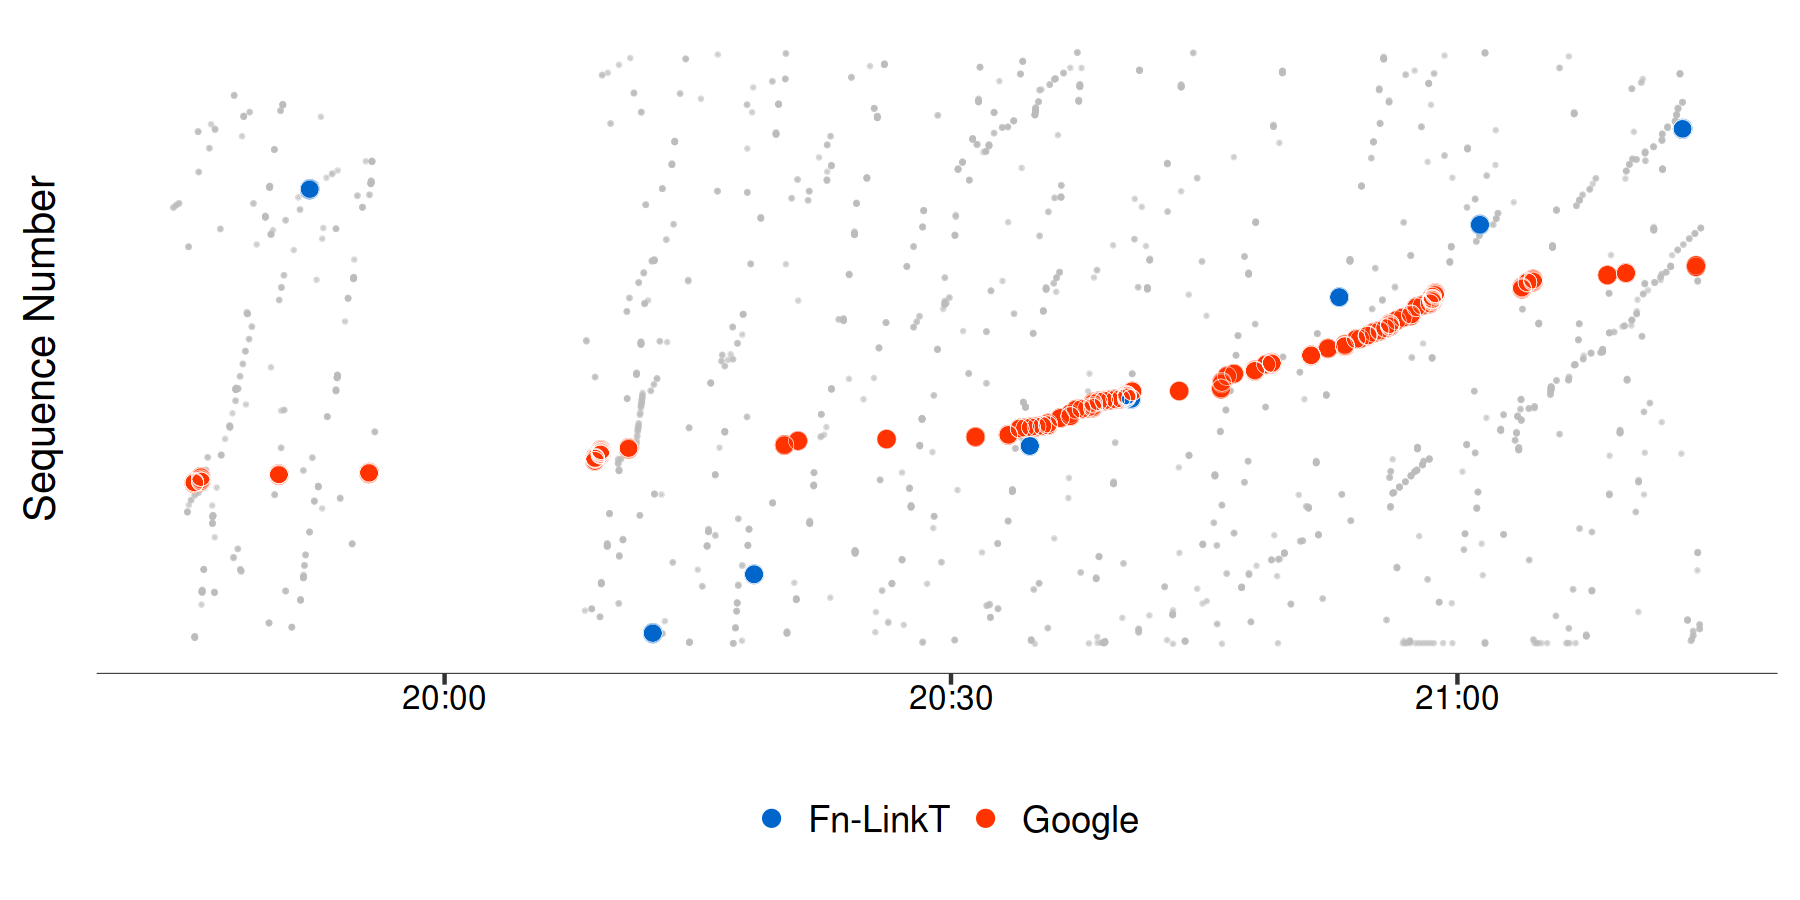
\includegraphics{images/home-sequence-time.png}
  \caption{Tree-map showing the volume of research conducted under each major themes and their sub-themes.}
  \label{figure:collection:home:sequence}
\end{figure}

Finally the sequence numbers are the most interesting part of the data collected. Though they don't uniquely identify the devices directly, along with timestamps they form visually discernible, unique patterns.
Figure \ref{figure:collection:home:sequence} we have isolated the two vendors and the probes with more than -70dBm and plotted their sequence numbers along with time. We can clearly see two devices which were present in the room. This shows the usefulness of the sequence number in estimating the actual devices around the sensors.
rotation of sequence numbers at 4096. This needs to be considered .
Figure \ref{figure:collection:home:samsung} shows a similar exploration of Samsung devices.
Though from the table \ref{table:collection:proberequest} it looked as if Samsung devices are randomising their MAC addresses, we can clearly that the diversity of MAC addresses are indeed unique devices which were far away from the sensor.
Though the results of this exploratory analysis has been positive the main challenge is to make sure these methods are feasible when dealing with more real-time, real world data.
We need to devise a more real world experiment to see frame lengths and signal strength work in a bigger data set for filtering out the noise. 

\begin{marginfigure}[-4cm]
  \forcerectofloat
  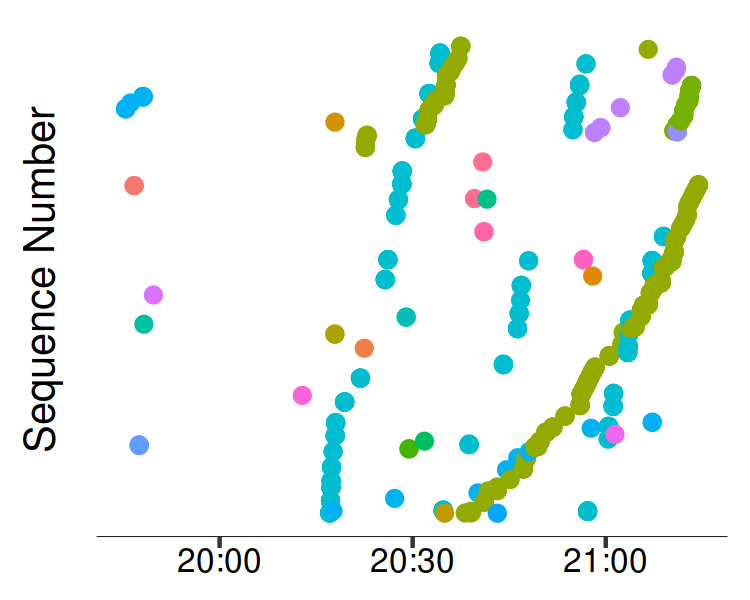
\includegraphics{images/home-samsung-google.png}
  \caption{Number of probe requests collected every minute on 15 October 2017}
  \label{figure:collection:home:samsung}
\end{marginfigure}
\marginnote{\textit{The colors show unique MAC addresses.} }

%------------------------------------------------------------------------------%
\subsection{University Hall}
%------------------------------------------------------------------------------%
This experiment was conducted to examine the previous results in a larger set of data in a more `real world' setting.
The specific goals are to validate the finding on signal strength corresponding to the distance from the sensor and to further examine the usefulness of the length parameter before collecting data on a busy retail setting.
Conducted in one of the main corridors - Southern cloisters of UCL with lot of pedestrian traffic.
There were also seating areas across the corridor where students work with their computers.
The area is also used heavily for lunch for large contingent of visitors.
Collected around 14750 probe requests collected and 652 users were counted walking around the sensors manually.

\begin{marginfigure}
  \forceversofloat
  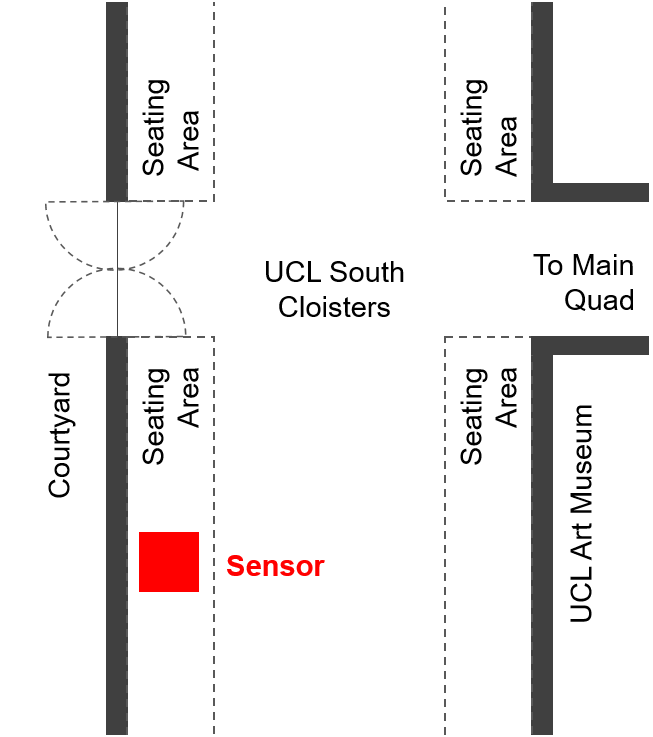
\includegraphics[trim={5 5 5 5},clip]{images/south-cloisters.png}
  \caption{Number of probe requests collected every minute on 15 October 2017}
  \label{figure:collection:ucl:config}
\end{marginfigure}
\marginnote{\textit{* Not to scale.} }

Major conclusion is that confirmation that Signal strength is still useful.
Length information is not that useful in certain standardised manufacturers.
At larger scales the manual counting is not possible without errors need to make a better alternative.

%------------------------------------------------------------------------------%
\subsection{Oxford Street}
%------------------------------------------------------------------------------%

Aim is to validate the filtering and clustering methodology against the scale and complexity of data collected in an open public area such as a retail high street.
We also aimed to find the algorithm which was best suited for the classification of signal strengths as 'low' and 'high' in order to filter out the background noise.
The data was collected at Oxford Street, London on 20 December 2017 from 12:30 to 13:00 hrs, Wi-Fi probe requests were collected using the sensor described in Section and pedestrian footfall was manually recorded using node-js based software, included in appendix.
Being located at one of the busiest retail locations in the United Kingdom, the Wi-Fi sensor captured approximately 60,000 probe requests during the half hour period; 3,722 people were manually recorded walking on the pavement during that time.
The surveyor positioned himself at the front of a store while carrying the sensor in a backpack and counted people walking by the store on the pavement (3m wide approximately) using a mobile phone.
The sensor was kept as close to the store window as possible, and the manual count was done as a cordon count in front of the store.

The analysis and use of this dataset is 

%------------------------------------------------------------------------------%
\subsection{Outputs from the experiments}
%------------------------------------------------------------------------------%

Probe requests are source of easy to collect rich information.
We identified list of useful information we can get from them.
We collected data in three phases starting from small isolated study, more footfall and real world retail location.
The first experiment showed that MAC address is not enough. Local mac addressed can be publicly registered as well.
Signal strength is crucial.
The broader UCL experiment in UCL corridor showed that though length information looked useful, it fails with apple devices since they are very similar to each other and lack any information elements. 
This gave us a good idea of what to collect in a field study. 
We collected data at Oxford street as a dataset for to be used as a starting point for any methodology we develop further.

%==============================================================================%


\section{Pilot Study}

As we see later in Section \ref{section:device-fingerprinting} the efficiency of the methods to clean and aggregate data not only depend on the noise and bias in the data itself but also on external factors such as, the configuration of the sensor in relation to the environment, the day of the week etc.
Thus the dataset captured in our initial experiments, though acts as a good starting point, cannot enable us to generalise our findings to all possible configurations.
This necessitates an even larger data collected over longer durations in challenging situations we usually find in real world conditions.
This was our primary motivation in conducting a pilot study collecting data at 5 locations across London.
The aim was to collect probe requests with information we found relevant in the initial experiments for every location surveyed for at least a full week so that we can understand any artifacts caused by the periodicity of the data.
We also wanted to collect data at all these locations in parallel for at least a week so that they can be compared to one other. 

\subsection{Methodology}

\begin{marginfigure}[2cm]
  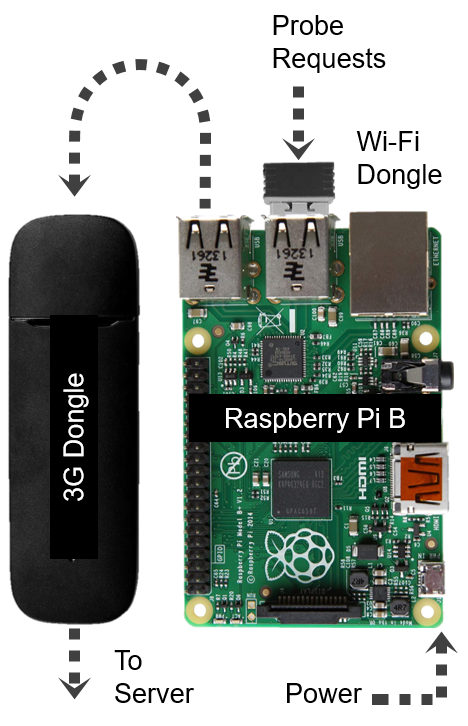
\includegraphics{images/pilot-hardware.png}
  \caption{Hardware setup used to collect data in the pilot studies.}
  \label{figure:collection:pilot:hardware}
\end{marginfigure}

The hardware setup for the sensors is illustrated in Figure \ref{figure:collection:pilot:hardware}.
It design of the hardware is not original as it is heavily influenced by the proprietary technology of the data partner for the Smart Street Sensor project albeit a much simpler form. 
The core of the hardware is the general purpose single board computer - Raspberry Pi Model B running Linux Operating system.
Two communication modules - 3G and Wi-Fi were connected to this machine via Universal Serial Bus interface.
3G modem was equipped with a SIM card which it uses to connect to the internet while the Wi-Fi modem is set to 'Monitor' mode.
The board takes power from an outlet and the software is pre installed with the operating system which resides in a Memory card.

The software used for the sensors consists of two parts - sensor software and server software.
The sensor software was written as a mix of Bash script and NodeJS.
Essentially these scripts use wireshark program to capture packets, parse them, anonymises the MAC address fields, adds the location information, encodes them into JavaScript Object Notation format and finally sends it to a server through Web-Socket protocol.
The code used at the sensor side is detailed in Appendix \ref{appendix:sensor:code}.
At the server side we have a similar NodeJS application which listens to the data sent over web sockets, parse them and saves them to a PostgreSQL database.
The server side code is detailed in Appendix \ref{} and schematic diagram for the whole process is shown in Figure \ref{figure:collection:pilot:schema}.
The information collected from each probe request at these locations are,

\begin{enumerate}[leftmargin=4em, rightmargin=2em]
  \itemsep-0.25em
  \item Time stamp at which it was received
  \item MAC address of the source device.
  \item Signal Strength of the packet.
  \item Total length of the packet.
  \item Sequence number of the packet.
  \item OUI part of MAC address.
  \item Location at which it is collected.
\end{enumerate}

\begin{figure*}
  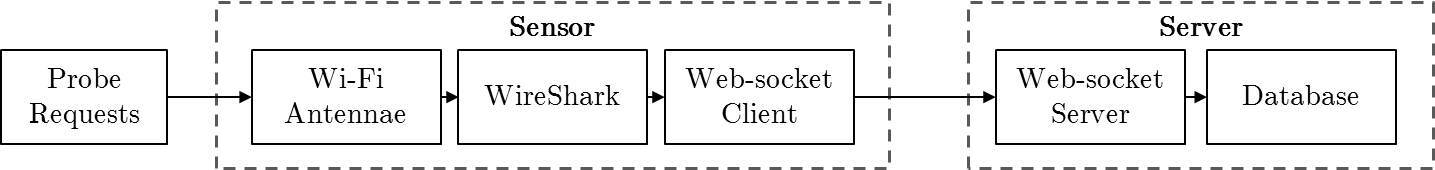
\includegraphics{images/pilot-study-system.jpeg}
  \caption{Schematic diagram showing the data collection process in the pilot study.}
  \label{figure:collection:pilot:schema}
\end{figure*}

The manual counting at these locations were done using a custom application \citet{bala2018}. The application was built for recording pedestrian footfall with precision and accuracy which was not possible when counted manually. The app records precise time stamp of every footfall with the precision of micro seconds which can be aggregated later at different time intervals. The code for the app is detailed in Section \ref{appendix:clicker}.

\subsection{Locations}

Five retail locations were chosen in consultation with the data partner for the pilot study keeping in mind their complexity and volume of footfall.
The sensors were installed at the locations in a phased manner and multiple manual counts were conducted at each location for 30 minute intervals.
The locations and their descriptions are summarised in Table \ref{table:collection:pilot:locations}.

\begin{figure}
  \centering
  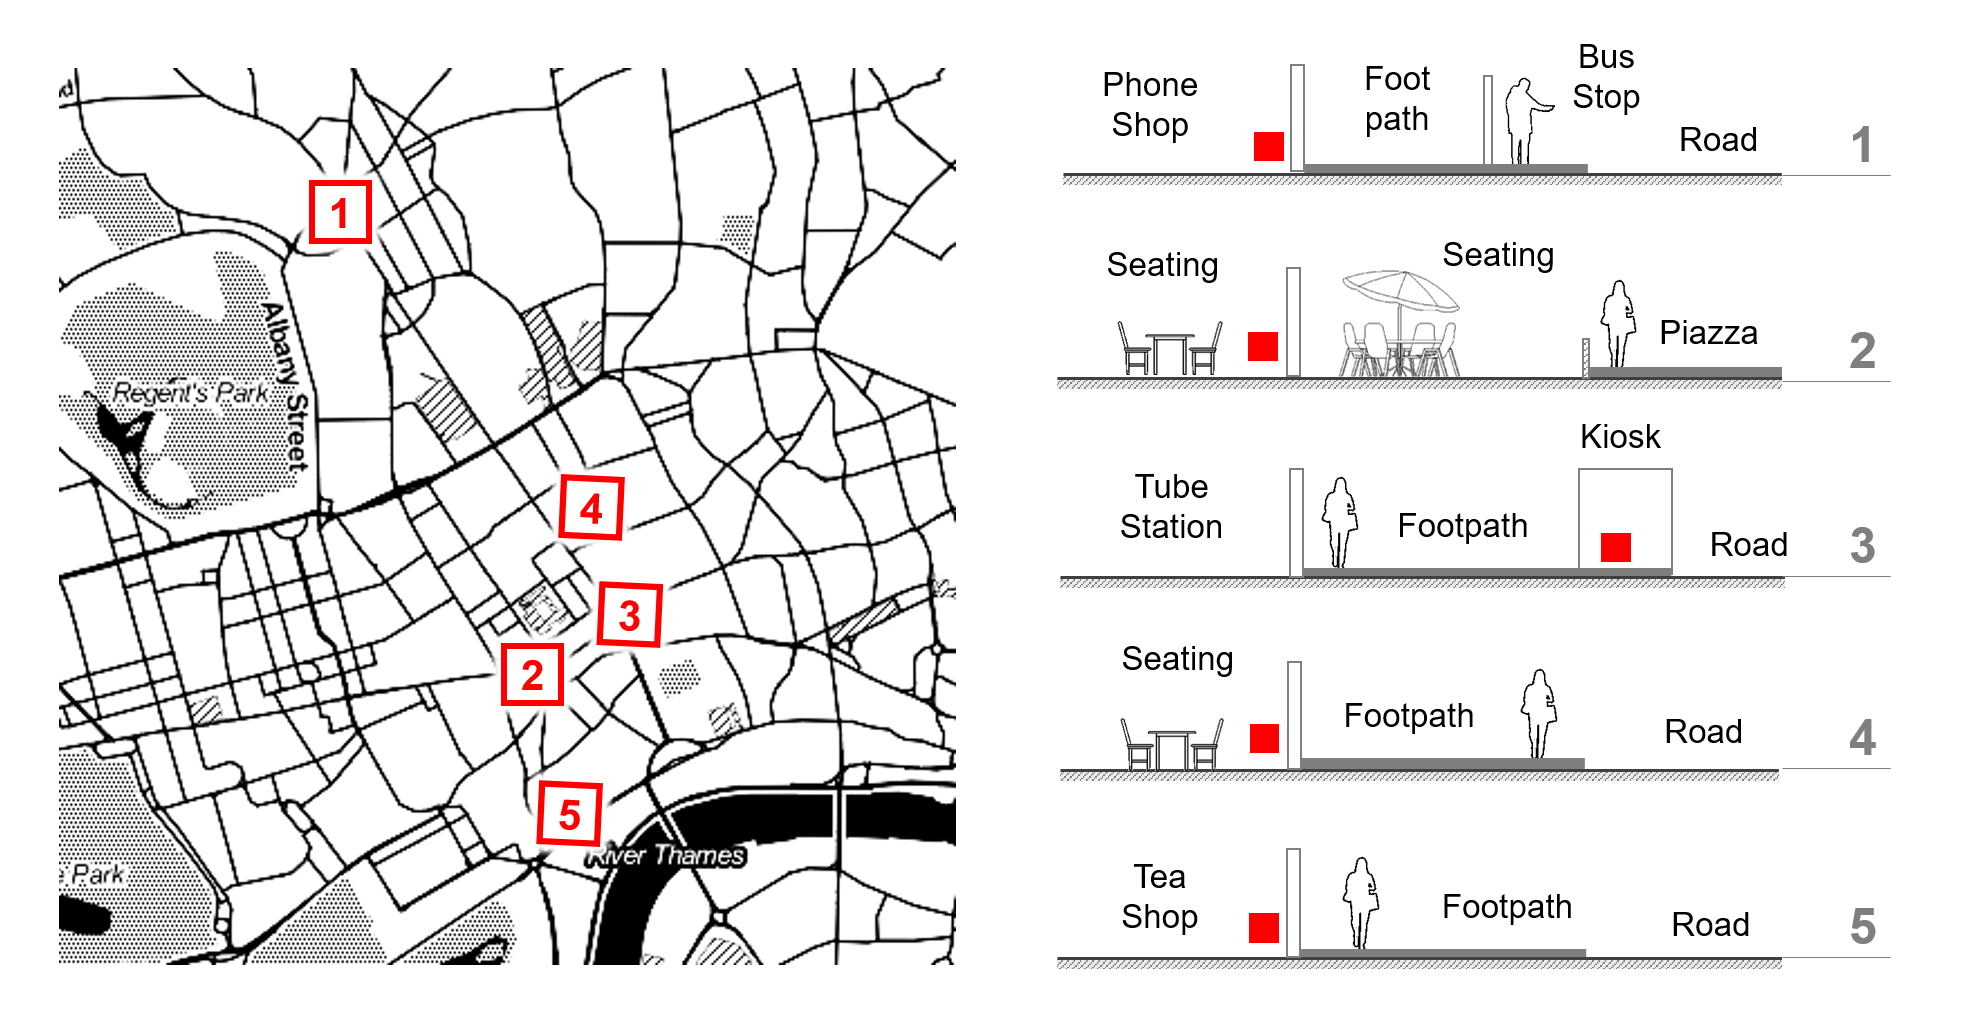
\includegraphics[trim={20 20 20 20},clip, width=\textwidth]{images/pilot-study-locations.png}
  \caption{Pilot study locations in London along with their corresponding sensor installation configurations.}
  \label{figure:literature:tech:timeline}
\end{figure}

\begin{itemize}[leftmargin=2em, rightmargin=2em]
  \item \textit{Location 1} is at the Camden high street in front of a mobile shop behind a bus stop. This location was chosen specifically because of the large amount of dwelling population at the bus stop and the stationary mobile devices inside the shop which is expected to create a large amount of noise along with the high footfall in the high street. The challenge here is to isolate the footfall from two sources of noises which are at equal distance from the sensor.
  \item \textit{Location 2} is at a square with a very low footfall but has a large amount of seating of the restaurant all around it. The challenge here is similar to that of the previous location but just that the volume of footfall is low which makes it one of the hardest locations for accurately estimating footfall.
  \item \textit{Location 3} is in front of Holborn station entrance in an information kiosk. This location was chosen for the really high volume from the station which is expected to cause noise. The challenge here is to be able to isolate the crowd inside the station from the footfall in the pavement.
  \item \textit{Location 4} is at a fast-food restaurant at a shopping center. The sensor has restaurant seating at one side and a pedestrian footfall at the other. The challenge here is that the stationary noise and the footfall are equidistant from the sensor.
  \item \textit{Location 5} is at the frontage of a shop at Strand with a mobile shop next door. This is the `cleanest' locations of all with only one clear source of noise which is at different distance from the footfall.
\end{itemize}

The sensors were operational through out February and March, while manual counts were conducted in these locations in half hour sessions on at least two different days.
The schedule of the data collection and the days at which the manual counting were done are shown in Figure \ref{figure:collection:pilot:schedule}.

\begin{figure*}
  
\includegraphics{images/pilot-study-schedule.png}
  \caption{Outline of the `Medium data toolkit' devised to collect, process, visualise and manage the Wi-Fi probe requests data}
  \label{figure:collection:pilot:schedule}
\end{figure*}

The survey was conducted for almost 2.5 months and about 33.5 million records were recorded which takes up to 1.8 GB of space on disk when encoded as text.
During the manual counts around 10,000 people were counted walking past these sensors.
A detailed account of the volume and velocity of data collected at these locations were given in Table \ref{table:collection:pilot:locations}.
The dataset collected was used extensively to develop and test the signal strength based filtering and sequence number based clustering methodology which are detailed in the Section \ref{section:device-fingerprinting}.

\begin{table} \footnotesize
\begin{center} \begin{tabular}{clllrr} \toprule
Id & Location & Type & Installation notes & Probes\textsuperscript{*} & Footfall\textsuperscript{**}\\
\midrule \addlinespace[0.2cm]
1 & Camden St.    & Phone Shop  & Bus stop in front         & 9.9 (297) & 3683 (33)\\ \addlinespace[0.1cm]
2 & St.Giles      & Restaurant  & Seating on both sides     & 3.9 (169) & 0346 (05)\\ \addlinespace[0.1cm]
3 & Holborn Stn.  & Info. Kiosk & Front of station entrance & 4.3 (303) & 2956 (46)\\ \addlinespace[0.1cm]
4 & Brunswick     & Fast Food   & Seating  on one side      & 3.4 (210) & 0960 (12)\\ \addlinespace[0.1cm]
5 & The Strand    & Tea Shop    & Phone shop next door      & 8.4 (382) & 1969 (21)\\ \addlinespace[0.05cm]
\bottomrule \end{tabular} \end{center}
\caption{Locations of data collection in the pilot study and the amount of data collected at each locations}
\label{table:collection:pilot:locations}
\end{table}
\marginnote[-1.5cm]{\textit{* Total probe requests in \(\times10^{6}\)(per minute)  ** Total footfall (per minute)}}


%==============================================================================%
\section{Smart Street Sensor Project}
%==============================================================================%
The Smart Street Sensor project is one of the most comprehensive studies carried out on consumer volume and characteristics in retail areas across the UK.
The project has been organised as a collaboration between the Consumer Data Research Centre, University College London (CDRC, UCL) and the Local Data Company (LDC).
The project was designed to serve as the first and unique comprehensive research into the patterns of retail activity in high streets of United Kingdom by measuring their real-time footfall from collecting Wi-Fi probe requests.
The data for the project was collected through sensors installed at around 1000 retail locations across UK.

The primary aim of the project is to improve our understanding of the dynamics of the high street retail climate in UK.
As we saw in our literature review, unlike online retail, this involves the quantification and measurement of human activity at small scales, such as high streets, which is already the subject of active research.
The key challenge in this area is the collection of data at the smallest scales possible with minimal resources while not infringing on people’s privacy.
This challenge when solved can provide immense value to the occupiers of the retail premises who want to improve revenues, to landlords who want to increase the value of the property, to local authorities who want to improve the vibrancy of the retail economy, and finally to investors and consumers within the retail industry.
The project also aims to facilitate decision making by these stakeholders, in addition to the tremendous opportunities for academic research.

\begin{marginfigure}[-2cm]
  \centering
  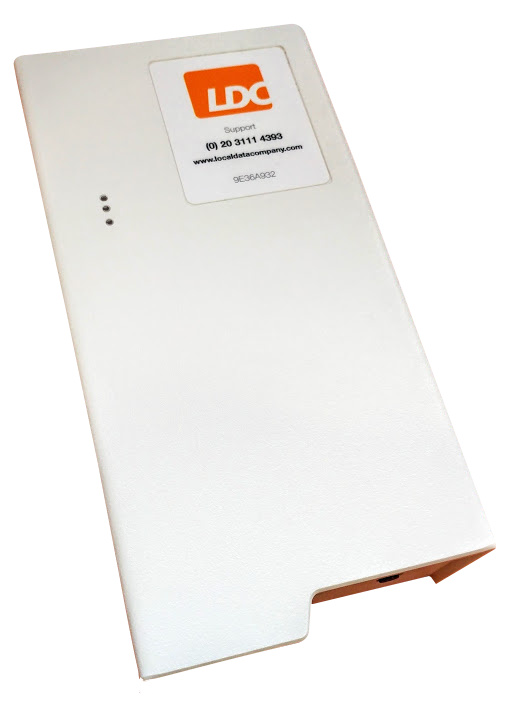
\includegraphics[height=3.5cm]{images/sss-hardware.jpg}
  \caption{Hardware setup used to collect data in the pilot studies.}
  \label{figure:collection:sss:hardware}
\end{marginfigure}

%------------------------------------------------------------------------------%
\subsection{Methodology}
%------------------------------------------------------------------------------%
As a first step, various locations for the study were identified by the CDRC to include a wide geographical spread, different demographic characteristics, and range of retail centre profiles.
Figure \ref{figure:collection:sss:locations} shows all the locations in the United Kingdom city-wise and Table \ref{table:collection:sss:locations} shows the regional distribution of the locations.

\begin{table}
  \footnotesize
  \begin{center} 
    \begin{tabular}{lr} 
      \toprule
      Region & Locations \\
      \midrule
      Greater London & 479 \\
      Scotland & 118 \\
      Yorkshire and the Humber & 114 \\
      South East & 103 \\
      North West & 98 \\
      South West & 87 \\
      East Midlands & 68 \\
      East Of England & 49 \\
      West Midlands & 39 \\
      North East & 26 \\
      Wales & 17 \\
      Northern Ireland & 2 \\
      \bottomrule
    \end{tabular}
  \end{center}
  \caption{Regional distribution of Smart Street Sensor locations across UK}
  \label{table:collection:sss:locations}
\end{table}

\begin{marginfigure}[6cm]
  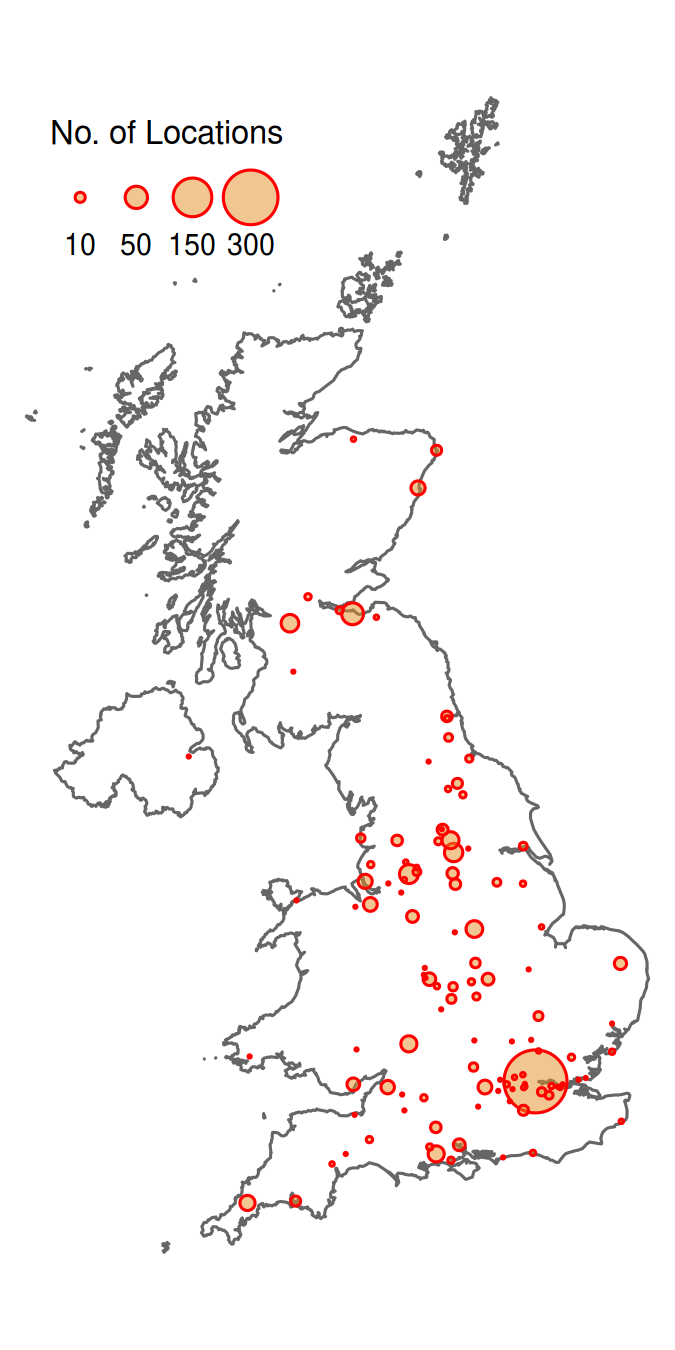
\includegraphics[trim = {0 20 0 0}, clip]{images/sss-locations.png}
  \caption{Distribution of locations with Smart Street Sensors installed.}
  \label{figure:collection:sss:locations}
\end{marginfigure}

We can see that the project has a strong London bias which along with other retail centres in the Greater London area, accounts for almost half of the locations.
We must also note that the locations are retail and any insight from the data needs to be looked at with a retail point of view.

A custom footfall counting technology using Wi-Fi sensors (Figure \ref{figure:collection:sss:hardware}) was also designed and developed by LDC, and the sensors were installed at the identified locations.
The sensor employs proprietary hardware and software, and monitors and records the probe requests sent by Wi-Fi enabled mobile devices present in its range.
In addition to this, the number of people walking by the sensor were counted manually for short time periods during the installation of the sensors at the corresponding locations.
The project aimed to combine these two sets of data to use as a proxy for estimating footfall at these locations.
The potentially personally identifiable information collected on the mobile devices are converted into a unique cryptographic hash at the sensor level and the data is sent to central server via encrypted channel for storage.
This data is then retrieved securely for the preparation of the commercial dashboards by LDC and for research purposes by CDRC.

The sensors are usually installed on a partnering retailer's shop window so that its range covers the pavement in front of the shops.
A typical configuration of a sensor in a location with respect to the premises and the pavement in front of it is illustrated in Figure \ref{figure:collection:sss:typical}.
There are also a small percentage (3\%) of the devices which are installed within large shops to monitor internal footfall.
Each device collects data independently and uploads the collected data to a central microsoft cloud facility (Azure) container at regular intervals of 5 minutes through a dedicated 3G mobile data connection.
The sensor hardware has been improved over the course of the project, and currently has built in failure prevention mechanisms such as, backup battery for power failures, automatic reboot capabilities, and in-device memory for holding data when the internet is not available.
The project began with the first sensor installation in July 2015, and has grown to an average of 650 daily active sensors as of January 2019, with a total of 1200 locations been involved in the project since its inception.
We have collected around 2TB of data comprising of around 73 billion probe requests.

\begin{figure*}
  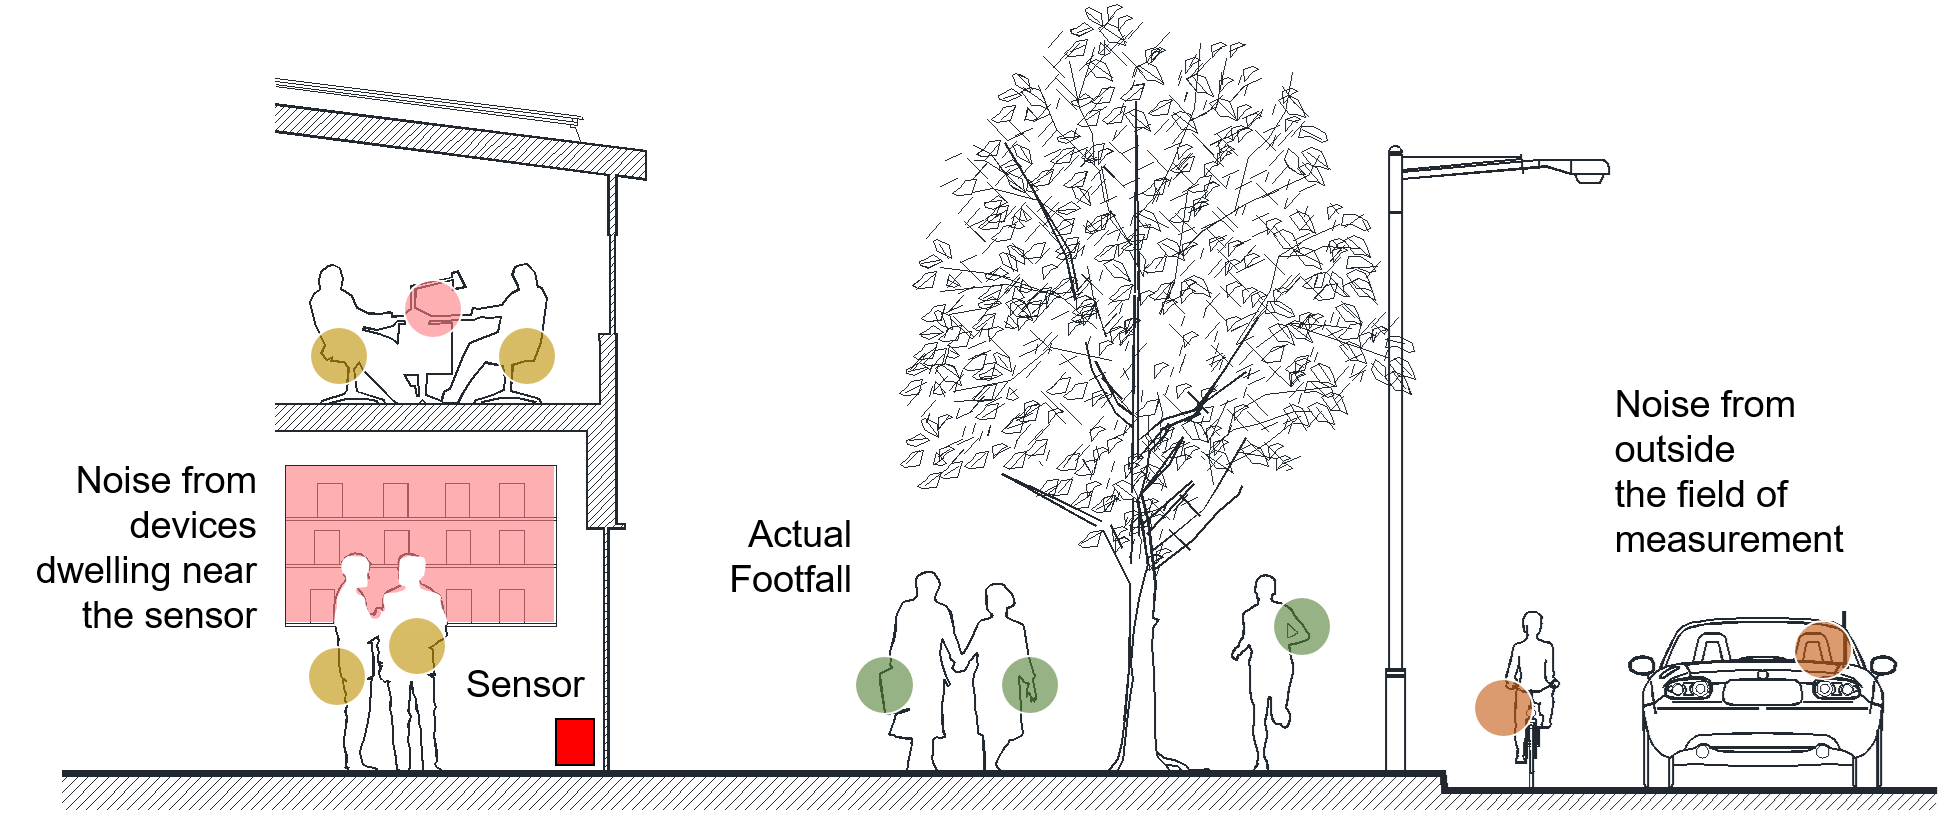
\includegraphics{images/sss.png}
  \caption{Cross section showing a typical installation of Smart Street Sensor in a retail frontage.}
  \label{figure:collection:sss:typical}
\end{figure*}

Due to the scale and the commercial nature of the project, the sensors collect fewer data per probe than the previous experiments.
The information collected by the Smart Street Sensors are the 5 minute interval when the probe request was collected, hashed MAC addresses and signal strength.
The probe requests within the same five minute intervals are aggregated by the MAC address, hence the signal strengths are aggregated to the minimum signal strength reported. 
Due to the longitudinal nature of the project, the data collection methods have changed over time as well.
The hardware was upgraded with more capabilities in early 2016, the interval they reboot at was adjusted several times in 2017, and finally, due to the MAC randomisation problem accentuated in the later part of 2017, the signal strength aggregation was changed from minimum to maximum in March 2018.
Essentially, the data have changed over time and we need to consider the changes while devising the methodologies for cleaning the data.


%------------------------------------------------------------------------------%
\section{Discussion}
%------------------------------------------------------------------------------%
In the previous sections we designed and implemented data collection processes to arrive at 3 different datasets - Small experiments, Pilot Study and Smart Street Sensor project. 
The small experiments were designed as way to collect as much data as possible from the probe requests for short periods of time aiming to collect small sets of comprehensive data under controlled conditions for exploratory purposes.
The pilot study extended this further by collecting data for a longer time in real world conditions aiming to validate the insights collected with the experiments and the methodologies we devise for the research.
The Smart Street Sensor is the most comprehensive study which collects very small focussed set of data at a national level for very long periods of time.
These datasets give us a well rounded set of data to set up our toolkit and devise out methodologies.
The summary of the datasets in terms of their characteristics is show in table \ref{table:collection:discussion:summary}.

Before we move on to develop methods to process the data into information on footfall in these locations, the crucial action is to look at the possible biases and uncertainties in these datasets arising due to the data collection methodology and from the broader context.
These form the framework on which built our data processing pipeline where we propose to solve each of these uncertainties in each step.

From our understanding of the data, we observe that the major sources of uncertainties are regarding the range of the sensor, the frequency at which mobile devices generate probe requests, the way and rate at which the mobile devices randomise their MAC addresses, the collisions caused due to the hashing of the MAC addresses and finally the gaps introduced by the failure of the sensors.
There is an inherent bias to these data caused by the mobile phone ownership in the population which varies across time, location and demography.
We discuss each of these uncertainties and biases in detail below,

\begin{table}
  \footnotesize
  \begin{center}
    \begin{tabular}{llllp{3cm}}
      \toprule
      Dataset & Locations & Time & Detail & Purpose\\
      \midrule
      \addlinespace[0.1cm]
      Small Experiments & 3 & 30 - 60 mins & High & Exploratory analysis\\
      \addlinespace[0.2cm]
      Pilot Study & 5 & 6 weeks* & Medium & Devising and calibrating methodologies\\
      \addlinespace[0.2cm]
      Smart Street Sensor & 1000* & 4 years* & Low & Real world insights\\
      \addlinespace[0.1cm]
      \bottomrule
    \end{tabular}
  \end{center}
  \caption{Summary of the collected data-sets.}
  \label{table:collection:discussion:summary}
\end{table}
\marginnote[-1cm]{\noindent\fontsize{7}{7}\textit{*approximate}}


%------------------------------------------------------------------------------%
\subsection{Range of the sensor}
%------------------------------------------------------------------------------%
The first and foremost uncertainty we face with wireless sensors such as Wi-Fi and Bluetooth is the delineation of the field of view of the sensor.
Though the Wi-Fi signals can be partly managed or restricted by manipulating their strength, there is no reliable way to precisely delineate a survey area for these sensors. 
The manipulation of signal strength can be done by installing metal shields around the sensors to block certain directions and prioritise others but the method cannot block out all the signals and will leave some uncertainty about where the probe requests are coming from.
Moreover, strength of the signal received from a mobile device by the Wi-Fi access point depends on numerous factors such as,

\begin{enumerate}
  \setlength{\itemindent}{2em}
  \itemsep-0.5em
  \item Distance between the mobile device and the Access Point.
  \item Thickness of the objects present in between them.
  \item Nature of obstructions such for e.g. metal vs glass
  \item Interference from other wireless devices.
  \item Power level of the transponder of the Access Point.
  \item Power level of the transponder of the Mobile device.
  \item Even atmospheric conditions such as humidity, temperature etc.
\end{enumerate}

The signal strength drops non-linearly when moving away from the access point as shown in Figure \ref{figure:collection:rssivsdist} and there is a \textit{close-range non-monotonicity} as well - where within 10 feet, A closer device can report lower signal strength than a farther one \citep{cisco2008}.
The relationship between the two is given by the equation \cite{rssieq},

\begin{equation}
  \log_{10}{d} = \frac{(P_o - F_m - P_r - (10 \times n \times \log_{10}{f}) + ( 30 \times n - 32.44))}{10\times n}
  \label{equation:rssi:hard}
\end{equation}

Where,

\noindent
\(d\) = distance - Sensitivity of the receiver \\
\(F_m\) = Fade Margin - Sensitivity of the receiver \\
\(n\) = Path-Loss Exponent, ranges from 2.7 to 4.3 \\
\(P_o\) = Signal power (dBm) at zero distance - Measured by testing \\
\(P_r\) = Signal power (dBm) at distance - Measured by testing \\
\(f\) = signal frequency in MHz - Specific to the hardware \\

\vspace{1em}

\begin{marginfigure}
  \forcerectofloat
  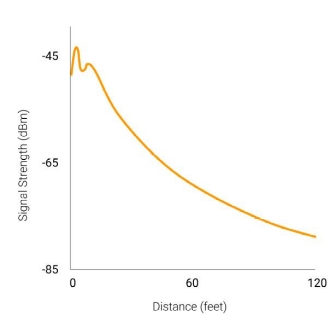
\includegraphics{images/rssi-vs-dist.jpeg}
  \caption{The decay of signal strength (RSSI) with respect to distance.}
  \label{figure:collection:rssivsdist}
\end{marginfigure}
\marginnote[0.5em]{\fontsize{7}{7}\textit{Source: Wi-Fi Location-Based Services, Cisco }}

All these factors vary widely in real world conditions at each location depending on where and how the sensors are installed.
They also vary widely over time due to changes in the context and vary across different directions at each location as well.
This makes it extremely difficult to model the distance between mobile device and the access point as a function of the received signal strength.
The equation \ref{equation:rssi:hard} can be approximated and simplified as,

\begin{equation}
  R = (-10 \times \log_{10}{d}) + A
  \label{equation:rssi:simple}
\end{equation}

Where \(R\) is the reported signal strength and \(A\) is the signal strength at 1 meter.
Though equation \ref{equation:rssi:simple} can help us to infer the distance of the mobile device roughly, the location wise uncertainty of this method makes it lose the meaning when compared across locations.

From the above we can conclude that it is almost impossible to delineate the field of measurement precisely and accurately by simple methods using the information present in the probe requests.
This leads to uncertainty in the data collected which needs to be resolved with explicit assumptions or specific methods to reduce the resulting noise.
We require a method to isolate this noise from data generated by devices within the field of measurement.
This methods needs to be independent of the micro site configuration, temporal changes in the context.

%------------------------------------------------------------------------------%
\subsection{Probe request frequency}
%------------------------------------------------------------------------------%
The second uncertainty we face is the frequency at which mobile devices generated the probe requests which varies wildly.
The number of probe requests generated from a mobile device depends on,

\begin{enumerate}
  \setlength{\itemindent}{2em}
  \itemsep-0.5em
  \item Manufacturer of the device. E.g. Samsung vs Apple
  \item Version of the software running on the device. E.g iOS 7 vs iOS 8
  \item State of the device. E.g. If it is already connected to internet? Has the location services been switched off?
  \item The number of access points already known to the device.
\end{enumerate}

Studies done by \citet{freud2015}\cite{freud2015} has shown that the number of probe requests generated by a mobile device vary widely across manufacturers such as Samsung, Apple and LG, across different state the devices are in such as charging, screen being on, Airplane mode being on etc and depends heavily on the number of access points known to the device.
It is also seen from our initial experiments that these probe requests are generated in short bursts rather than being generated at regular intervals.
This makes predicting a base factor for calculating a number of mobile devices based on the number of probe requests received much more complex.
The variety of device models available and the pace of change in software that run these models further complicates this.
Though we can simply aggregate these probe requests based on the unique information on them, in absence of such information it becomes extremely critical.
We to consider this uncertainty in detail while making any simple assumptions on the relationship between number of probe requests and the number of mobile devices that generated them.

%------------------------------------------------------------------------------%
\subsection{MAC address randomisation}
%------------------------------------------------------------------------------%
Randomisation of MAC address is one of the recent uncertainty introduced in the data.
As we saw in section \ref{wifi-as-source-of-data} MAC address is the unique identifier for each mobile device and we aggregate the footfall numbers based on this.
Since the probe requests are transmitted unencrypted and can be received by any access point, this is one of the biggest leak of personal data which occurs in the Wi-Fi based communications.
Modern mobile devices solve this problem by using a randomised MAC address for the probe requests which can result in large over estimation of number of mobile devices in the vicinity.

\begin{marginfigure}
  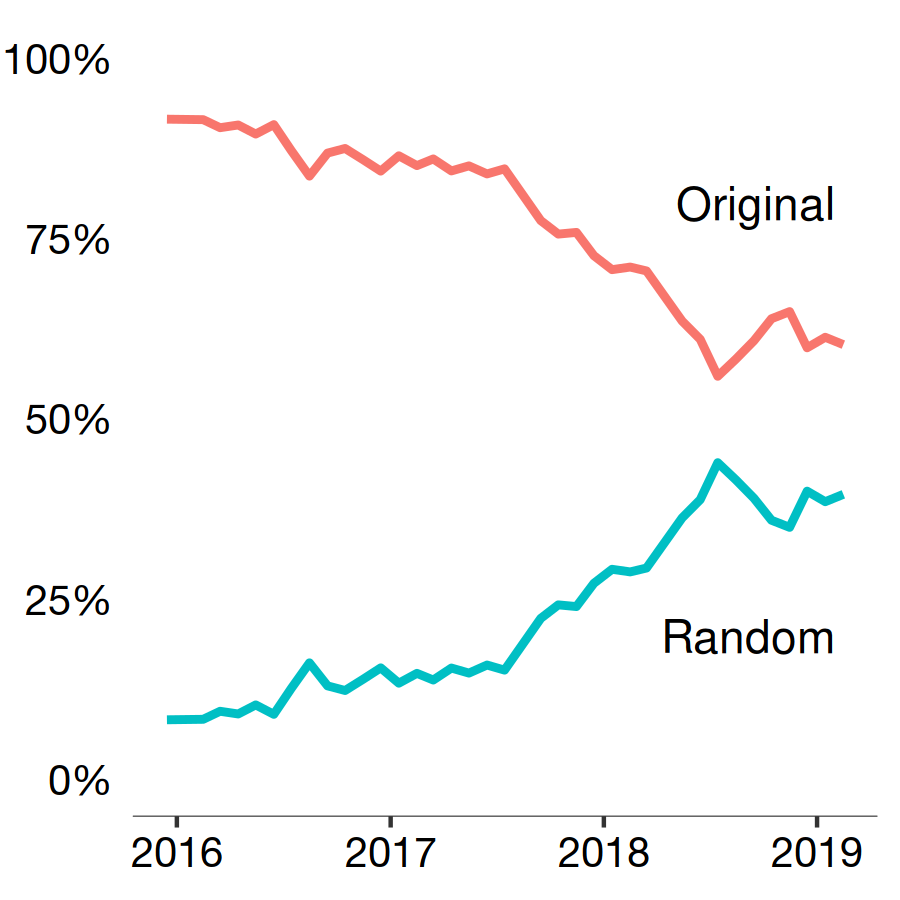
\includegraphics{images/mac-randomisation.png}
  \caption{Increase in the share of randomised MAC addresses compared to non-randomised original ones over the years.}
  \label{figure:collection:macrandom}
\end{marginfigure}
\marginnote{\fontsize{7}{7}\textit{From data collected at Regent Street, Cambridge.}}

The method of randomisation and the frequency varies widely between device manufacturers and also changes as new versions of the software are released.
This seriously affects the usefulness of the data long term where methods designed to overcome this randomisation can be rendered inefficient in the future.
Figure \ref{figure:collection:macrandom} shows the increase in the share of randomised MAC addresses since 2015.
We can observe that in addition to the overall upward trend there are bursts of increase around late 2016 and 2017 which coincides with the release of new mobile operating systems.
This makes it necessary for devising a method to overcome MAC randomisation problem to be able to uniquely fingerprint devices so that they can be aggregated together.
As we saw in our literature review, this is also one of the major opportunities in research on human mobility using Wi-Fi data.

%------------------------------------------------------------------------------%
\subsection{Mobile Device Ownership}
%------------------------------------------------------------------------------%
One of the major external bias in all the datasets collected from mobile devices is the overall volume and nature of the ownership of these devices.
The ownership of mobile devices, specifically Wi-Fi enabled ones, have been on the rise since 2005.
Though mobile ownership has reached unprecedented level in recent years, there is still an underlying increasing trend present in the ownership of these devices which manifests itself in the collected data.
Moreover the mobile ownership varies widely between demography of age and geography as well. 
Figure \ref{figure:collection:ownership} shows the mobile ownership across age groups in UK from 2012 to 2018.
We can observe that the older age groups are under-represented in our data.
This needs to be taken into consideration while using this data for extrapolating demographic conclusions out of it.
In addition to this, the overall upward trend needs to be adjusted assuming 1\% increase monthly and 0.2\% weekly when using this data across long periods of time.

\begin{marginfigure}
  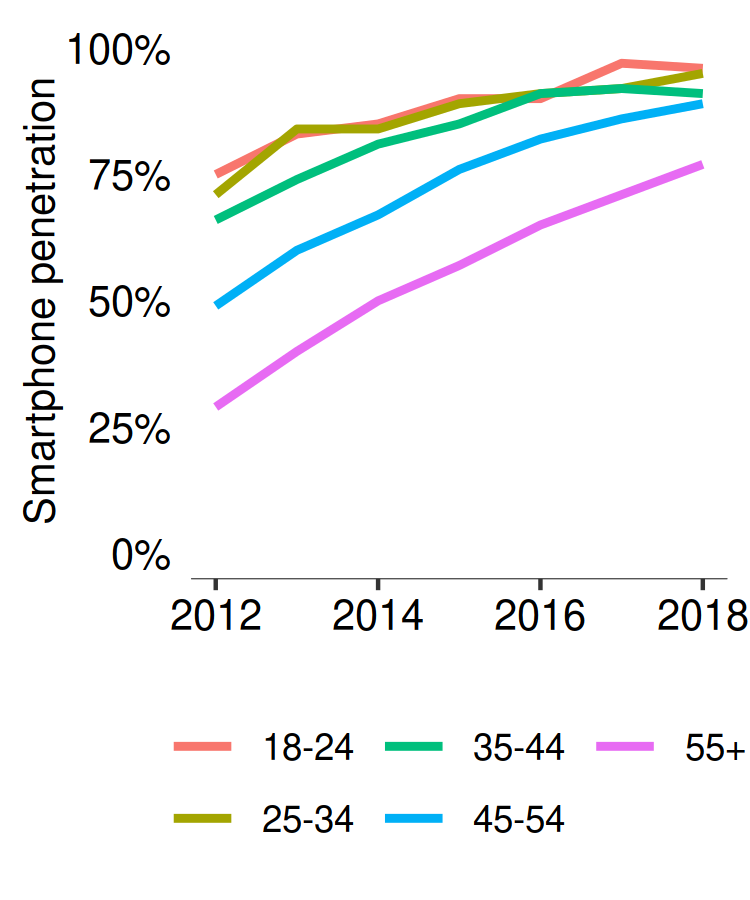
\includegraphics{images/mobile-ownership.png}
  \caption{Smartphone penetration by age group in United Kingdom (2012-18)}
  \label{figure:collection:ownership}
\end{marginfigure}
\marginnote{\fontsize{7}{7}\textit{Source: UK edition, Deloitte Global Mobile Consumer Survey, }}



%------------------------------------------------------------------------------%
\subsection{Missing Data}
%------------------------------------------------------------------------------%
Being collected by distributed set of sensors located in busy real-world scenarios, the data has a large number of gaps as well.
These gaps are caused by various reasons such as, failure of the sensor hardware and software, failure in internet connectivity to send the data back, External factors such as store closures which can cause power loss, regular disruptions such as software update and maintenance and finally other factors such as unauthorised tampering and unplugging of the sensor.
This is leads to a dataset which contains several small and medium sized gaps as shown in Figure \ref{figure:toolkit:veracity:gaps}.
More over, the Smart Street Sensor project is implemented and managed with commercial motive, the sensors are installed and uninstalled at locations as retail partners join and leave the project.
This leads to an uneven availability of data across locations over longer time periods which creates challenges while aggregating data across locations.
We need to implement a methodology to fill in these gaps which considers the periodic patterns in the data.
We also need to devise a measure for aggregating the counts across locations which removes the bias introduced by long term gaps in data.

%------------------------------------------------------------------------------%
\subsection{MAC address collisions}
%------------------------------------------------------------------------------%
Finally, from the initial analysis we have observed that there are few instances of collisions occurring in the hashed MAC addresses.
This has been observed as unique hashed MAC addresses appear at different locations within a short period of time which cannot be explained by the physical travel by the user between these locations.
These collisions are caused by the limitation of the hashing algorithm used and exist only in very large amounts of data.
It is important to note that this collision are specific to non-randomised MAC addresses as we don't expect any consistency within the randomised ones.
Even though this is an inevitable side effect of the hashing process, the probability of such occurrence is very low and is calculated as \(2^{-n}\), where \(n\) is the number of bits in the output of the hashing algorithm.
The total number of estimated collisions between \(m\) unique values is given by, \(2^{-n} \times {m \choose 2}\)\cite{estcollision}.
This translates to around 100 collisions across a million unique devices with a 32 bit algorithm and 2 collisions across 10 Billion devices when using a 64 bit algorithm. 
Though these collisions might cause issues in granular mobility models, for long term and broad studies where we don't track individual devices, they can be safely ignored.

